
\section{Vektorieller Netzwerkanalysator (VNA) I}
\label{section:vna_1}
\begin{frame}%STARTCONTENT

\begin{columns}
    \begin{column}{0.48\textwidth}
    \begin{itemize}
  \item Ein einfaches Multimeter kann keine frequenzabhängigen Widerstände messen
  \item Dazu wird ein \emph{vektorieller Netzwerkanalysator (VNA)} verwendet
  \end{itemize}

    \end{column}
   \begin{column}{0.48\textwidth}
       \begin{itemize}
  \item Aktives Messgerät
  \item Misst das Verhältnis von Spannung und Strom bei einer Frequenz
  \item Oft kann ein Frequenzbereich angegeben werden
  \end{itemize}

   \end{column}
\end{columns}

\end{frame}

\begin{frame}
\frametitle{Anwendungen}
\begin{columns}
    \begin{column}{0.48\textwidth}
    \begin{itemize}
  \item Große und kleine Widerstände eines Schwingkreis
  \item Resonanzfrequenz eines Schwingkreis
  \item Filterverhalten
  \item Impedanzmessung
  \item Stehwellenverhältnisse
  \end{itemize}

    \end{column}
   \begin{column}{0.48\textwidth}
       
\begin{figure}
    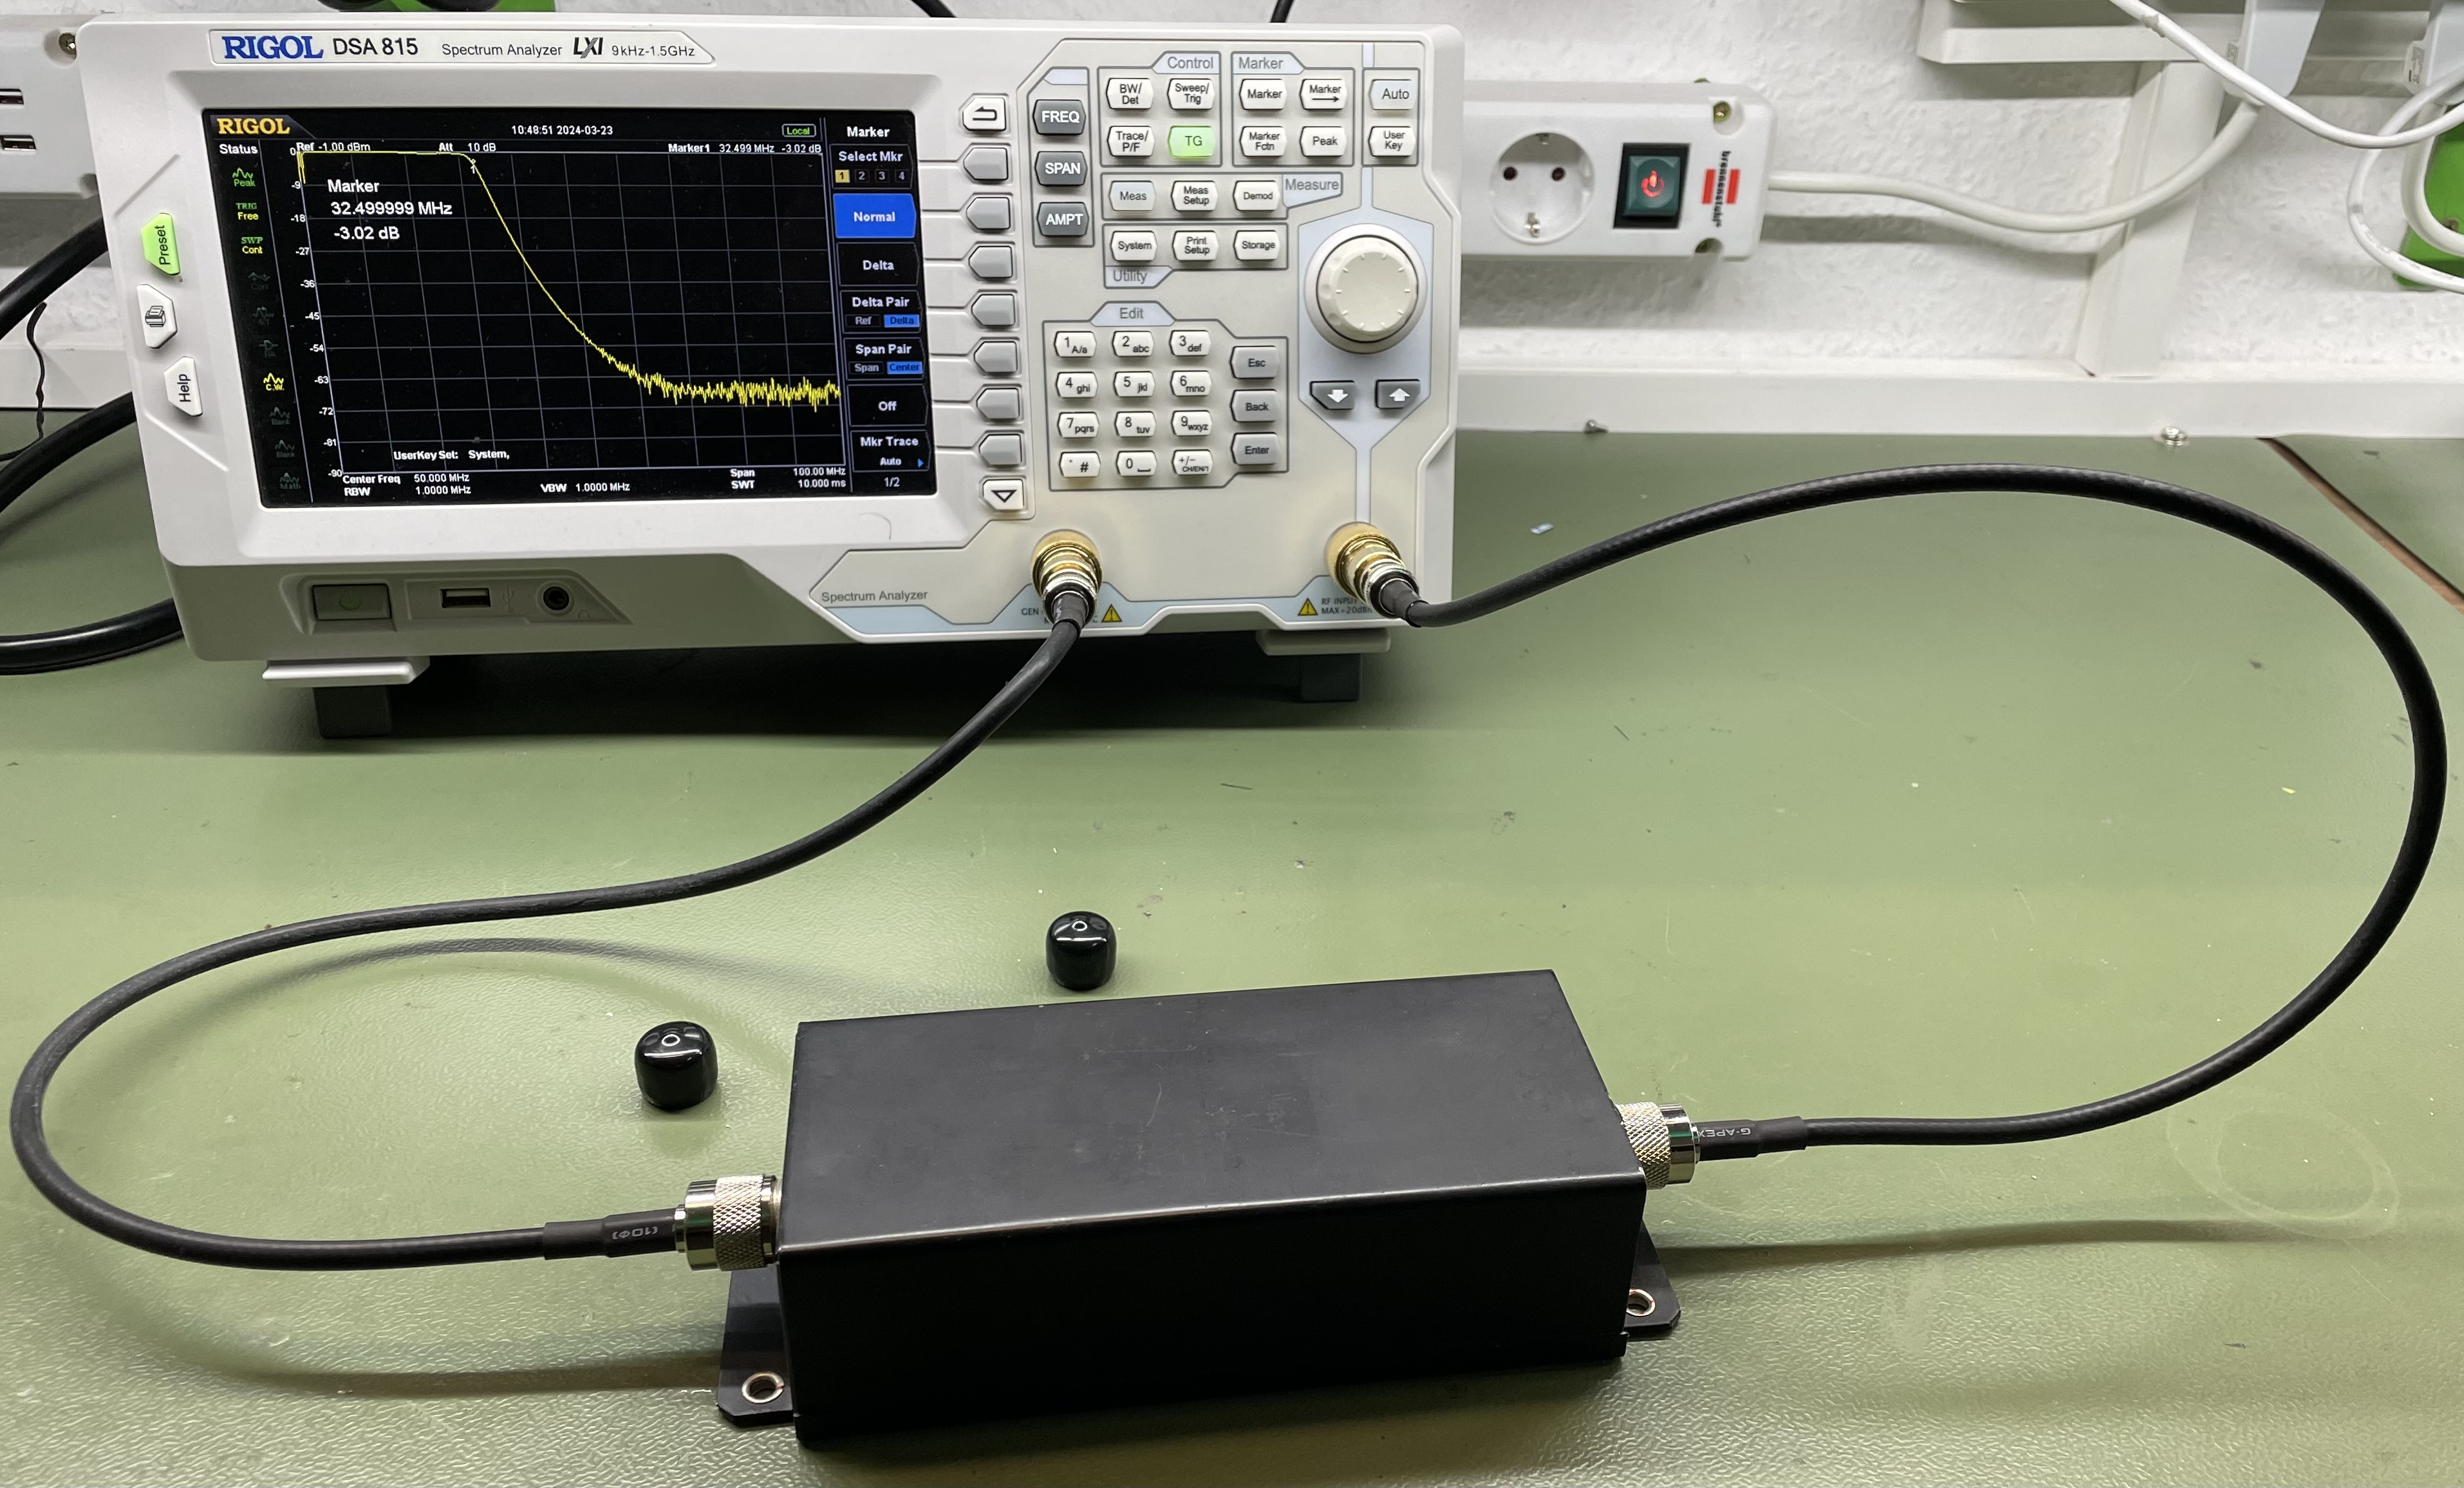
\includegraphics[width=0.85\textwidth]{foto/201}
    \caption{\scriptsize Messung eines Tiefpassfilters mit Grenzfrequenz bei 30MHz}
    \label{e_vna_tiefpassmessung}
\end{figure}

   \end{column}
\end{columns}

\end{frame}

\begin{frame}
\only<1>{
\begin{QQuestion}{EI201}{Wozu wird ein \glqq vektorieller Netzwerkanalysator\grqq{} (VNA) beispielsweise verwendet?}{Zur Bestimmung des Erdungswiderstandes einer Amateurfunkstation.}
{Zum Aufzeichnen des zeitlichen Verlaufs schneller Wechselströme.}
{Zur Überprüfung der Frequenzreinheit eines Senders.}
{Zur genaueren Bestimmung von Resonanzfrequenzen und Impedanzen von Schwingkreisen und Antennen.}
\end{QQuestion}

}
\only<2>{
\begin{QQuestion}{EI201}{Wozu wird ein \glqq vektorieller Netzwerkanalysator\grqq{} (VNA) beispielsweise verwendet?}{Zur Bestimmung des Erdungswiderstandes einer Amateurfunkstation.}
{Zum Aufzeichnen des zeitlichen Verlaufs schneller Wechselströme.}
{Zur Überprüfung der Frequenzreinheit eines Senders.}
{\textbf{\textcolor{DARCgreen}{Zur genaueren Bestimmung von Resonanzfrequenzen und Impedanzen von Schwingkreisen und Antennen.}}}
\end{QQuestion}

}
\end{frame}

\begin{frame}
\only<1>{
\begin{QQuestion}{EI202}{Wie ermittelt man die Resonanzfrequenz eines Schwingkreises? Man ermittelt sie~...}{durch Messung von $L$ und $C$ und Berechnung oder z.~B. mit einem vektoriellen Netzwerkanalysator (VNA).}
{mit einem Frequenzmesser oder einem Oszilloskop.}
{mit einem Digital-Multimeter in der Stellung Frequenzmessung.}
{mit Hilfe der S-Meter-Anzeige bei Anschluss des Schwingkreises an den Empfängereingang.}
\end{QQuestion}

}
\only<2>{
\begin{QQuestion}{EI202}{Wie ermittelt man die Resonanzfrequenz eines Schwingkreises? Man ermittelt sie~...}{\textbf{\textcolor{DARCgreen}{durch Messung von $L$ und $C$ und Berechnung oder z.~B. mit einem vektoriellen Netzwerkanalysator (VNA).}}}
{mit einem Frequenzmesser oder einem Oszilloskop.}
{mit einem Digital-Multimeter in der Stellung Frequenzmessung.}
{mit Hilfe der S-Meter-Anzeige bei Anschluss des Schwingkreises an den Empfängereingang.}
\end{QQuestion}

}
\end{frame}

\begin{frame}
\only<1>{
\begin{QQuestion}{EI203}{Mit welchem Messgerät können Impedanzen, Blindwiderstände und Stehwellenverhältnisse direkt gemessen werden?}{digitales Speicheroszilloskop}
{analoges Multimeter}
{vektorieller Netzwerkanalysator}
{True RMS-Voltmeter}
\end{QQuestion}

}
\only<2>{
\begin{QQuestion}{EI203}{Mit welchem Messgerät können Impedanzen, Blindwiderstände und Stehwellenverhältnisse direkt gemessen werden?}{digitales Speicheroszilloskop}
{analoges Multimeter}
{\textbf{\textcolor{DARCgreen}{vektorieller Netzwerkanalysator}}}
{True RMS-Voltmeter}
\end{QQuestion}

}
\end{frame}

\begin{frame}
\only<1>{
\begin{QQuestion}{EI204}{Wozu ist ein vektorieller Netzwerkanalysator (VNA) beispielsweise geeignet?}{Datenübertragungsraten in Netzwerken erfassen.}
{Messen von Impedanzen.}
{Direkte Messung der Sendeleistung.}
{Messen von Oberschwingungen.}
\end{QQuestion}

}
\only<2>{
\begin{QQuestion}{EI204}{Wozu ist ein vektorieller Netzwerkanalysator (VNA) beispielsweise geeignet?}{Datenübertragungsraten in Netzwerken erfassen.}
{\textbf{\textcolor{DARCgreen}{Messen von Impedanzen.}}}
{Direkte Messung der Sendeleistung.}
{Messen von Oberschwingungen.}
\end{QQuestion}

}
\end{frame}

\begin{frame}
\frametitle{Kalibrierung}
\begin{itemize}
  \item Vor der Benutzung kalibrieren
  \item Zustand \emph{offen}: unendlicher Widerstand
  \item Zustand \emph{Kurzschluss}: Widerstand nahe Null
  \item Zustand \emph{angepasst}: z.B. mit 50 Ω Widerstand sollte ein SWR von 1 angezeigt werden
  \end{itemize}
\end{frame}

\begin{frame}
\only<1>{
\begin{QQuestion}{EI205}{Welche Maßnahme ist vor Gebrauch eines vektoriellen Netzwerkanalysators (VNA) zusammen mit dem Messaufbau durchzuführen?}{Rauschunterdrückung aktivieren}
{Nullpunktabgleich}
{Einstellen der Triggerschwelle}
{Kalibrierung}
\end{QQuestion}

}
\only<2>{
\begin{QQuestion}{EI205}{Welche Maßnahme ist vor Gebrauch eines vektoriellen Netzwerkanalysators (VNA) zusammen mit dem Messaufbau durchzuführen?}{Rauschunterdrückung aktivieren}
{Nullpunktabgleich}
{Einstellen der Triggerschwelle}
{\textbf{\textcolor{DARCgreen}{Kalibrierung}}}
\end{QQuestion}

}
\end{frame}

\begin{frame}
\only<1>{
\begin{QQuestion}{EI206}{Sie ermitteln die Resonanzfrequenz und die Impedanz ihrer selbstgebauten Antennen mit Hilfe eines vektoriellen Netzwerkanalysators (VNA). Wie könnten Sie die Funktion des Gerätes vorher prüfen?}{Durch Beschalten des Messeingangs am VNA mit einem Abschlusswiderstand. Das angezeigte SWR sollte im gesamten Frequenzbereich größer als 2 sein.}
{Durch Prüfen der Anzeigewerte in den Betriebszuständen Leerlauf und Anpassung. Der Messanschluss des Gerätes darf keinesfalls kurzgeschlossen werden.}
{Durch Prüfen der Anzeigewerte in den Betriebszuständen Kurzschluss, Leerlauf und Anpassung. Das SWR sollte bei Anpassung nahe bei 1, bei Kurzschluss und Leerlauf unendlich sein.}
{Durch Beschalten des Messeingangs am VNA mit einem Blindwiderstand. Der Anzeigewert des SWR muss bei allen Frequenzen nahe bei 1 sein.}
\end{QQuestion}

}
\only<2>{
\begin{QQuestion}{EI206}{Sie ermitteln die Resonanzfrequenz und die Impedanz ihrer selbstgebauten Antennen mit Hilfe eines vektoriellen Netzwerkanalysators (VNA). Wie könnten Sie die Funktion des Gerätes vorher prüfen?}{Durch Beschalten des Messeingangs am VNA mit einem Abschlusswiderstand. Das angezeigte SWR sollte im gesamten Frequenzbereich größer als 2 sein.}
{Durch Prüfen der Anzeigewerte in den Betriebszuständen Leerlauf und Anpassung. Der Messanschluss des Gerätes darf keinesfalls kurzgeschlossen werden.}
{\textbf{\textcolor{DARCgreen}{Durch Prüfen der Anzeigewerte in den Betriebszuständen Kurzschluss, Leerlauf und Anpassung. Das SWR sollte bei Anpassung nahe bei 1, bei Kurzschluss und Leerlauf unendlich sein.}}}
{Durch Beschalten des Messeingangs am VNA mit einem Blindwiderstand. Der Anzeigewert des SWR muss bei allen Frequenzen nahe bei 1 sein.}
\end{QQuestion}

}
\end{frame}%ENDCONTENT
